\documentclass{article}[18pt]
%\ProvidesPackage{format}
%Page setup
\usepackage[utf8]{inputenc}
\usepackage[margin=0.7in]{geometry}
\usepackage{parselines} 
\usepackage[english]{babel}
\usepackage{fancyhdr}
\usepackage{titlesec}
\hyphenpenalty=10000

\pagestyle{fancy}
\fancyhf{}
\rhead{Sam Robbins}
\rfoot{Page \thepage}

%Characters
\usepackage{amsmath}
\usepackage{amssymb}
\usepackage{gensymb}
\newcommand{\R}{\mathbb{R}}

%Diagrams
\usepackage{pgfplots}
\usepackage{graphicx}
\usepackage{tabularx}
\usepackage{relsize}
\pgfplotsset{width=10cm,compat=1.9}
\usepackage{float}

%Length Setting
\titlespacing\section{0pt}{14pt plus 4pt minus 2pt}{0pt plus 2pt minus 2pt}
\newlength\tindent
\setlength{\tindent}{\parindent}
\setlength{\parindent}{0pt}
\renewcommand{\indent}{\hspace*{\tindent}}

%Programming Font
\usepackage{courier}
\usepackage{listings}
\usepackage{pxfonts}

%Lists
\usepackage{enumerate}
\usepackage{enumitem}

% Networks Macro
\usepackage{tikz}


% Commands for files converted using pandoc
\providecommand{\tightlist}{%
	\setlength{\itemsep}{0pt}\setlength{\parskip}{0pt}}
\usepackage{hyperref}

% Get nice commands for floor and ceil
\usepackage{mathtools}
\DeclarePairedDelimiter{\ceil}{\lceil}{\rceil}
\DeclarePairedDelimiter{\floor}{\lfloor}{\rfloor}

% Allow itemize to go up to 20 levels deep (just change the number if you need more you madman)
\usepackage{enumitem}
\setlistdepth{20}
\renewlist{itemize}{itemize}{20}

% initially, use dots for all levels
\setlist[itemize]{label=$\cdot$}

% customize the first 3 levels
\setlist[itemize,1]{label=\textbullet}
\setlist[itemize,2]{label=--}
\setlist[itemize,3]{label=*}

% Definition and Important Stuff
% Important stuff
\usepackage[framemethod=TikZ]{mdframed}

\newcounter{theo}[section]\setcounter{theo}{0}
\renewcommand{\thetheo}{\arabic{section}.\arabic{theo}}
\newenvironment{important}[1][]{%
	\refstepcounter{theo}%
	\ifstrempty{#1}%
	{\mdfsetup{%
			frametitle={%
				\tikz[baseline=(current bounding box.east),outer sep=0pt]
				\node[anchor=east,rectangle,fill=red!50]
				{\strut Important};}}
	}%
	{\mdfsetup{%
			frametitle={%
				\tikz[baseline=(current bounding box.east),outer sep=0pt]
				\node[anchor=east,rectangle,fill=red!50]
				{\strut Important:~#1};}}%
	}%
	\mdfsetup{innertopmargin=10pt,linecolor=red!50,%
		linewidth=2pt,topline=true,%
		frametitleaboveskip=\dimexpr-\ht\strutbox\relax
	}
	\begin{mdframed}[]\relax%
		\centering
		}{\end{mdframed}}



\newcounter{lem}[section]\setcounter{lem}{0}
\renewcommand{\thelem}{\arabic{section}.\arabic{lem}}
\newenvironment{definition}[1][]{%
	\refstepcounter{lem}%
	\ifstrempty{#1}%
	{\mdfsetup{%
			frametitle={%
				\tikz[baseline=(current bounding box.east),outer sep=0pt]
				\node[anchor=east,rectangle,fill=blue!20]
				{\strut Definition};}}
	}%
	{\mdfsetup{%
			frametitle={%
				\tikz[baseline=(current bounding box.east),outer sep=0pt]
				\node[anchor=east,rectangle,fill=blue!20]
				{\strut Definition:~#1};}}%
	}%
	\mdfsetup{innertopmargin=10pt,linecolor=blue!20,%
		linewidth=2pt,topline=true,%
		frametitleaboveskip=\dimexpr-\ht\strutbox\relax
	}
	\begin{mdframed}[]\relax%
		\centering
		}{\end{mdframed}}
	
\newcounter{prob}[section]\setcounter{prob}{0}
\renewcommand{\theprob}{\arabic{section}.\arabic{lem}}
\newenvironment{problem}[1][]{%
	\refstepcounter{prob}%
	\ifstrempty{#1}%
	{\mdfsetup{%
			frametitle={%
				\tikz[baseline=(current bounding box.east),outer sep=0pt]
				\node[anchor=east,rectangle,fill=orange!20]
				{\strut Problem};}}
	}%
	{\mdfsetup{%
			frametitle={%
				\tikz[baseline=(current bounding box.east),outer sep=0pt]
				\node[anchor=east,rectangle,fill=orange!20]
				{\strut Problem:~#1};}}%
	}%
	\mdfsetup{innertopmargin=10pt,linecolor=orange!20,%
		linewidth=2pt,topline=true,%
		frametitleaboveskip=\dimexpr-\ht\strutbox\relax
	}
	\begin{mdframed}[]\relax%
	}{\end{mdframed}}
	
% Styling Pseudocode
\lstset{language=C,
	basicstyle=\ttfamily,
	keywordstyle=\bfseries,
	showstringspaces=false,
	morekeywords={if, else, then, print, end, for, do, while, Let},
	tabsize=4,
	mathescape=true,
	escapechar=£,
	numbers=left,
	stepnumber=1,
	frame=top,
	frame=bottom
}

\usepackage{caption}
\DeclareCaptionFormat{listing}{\rule{\dimexpr\textwidth+17pt\relax}{0.4pt}\par\vskip1pt#1#2#3}
\captionsetup[lstlisting]{format=listing,singlelinecheck=false, margin=0pt, font={sf},labelsep=space,labelfont=bf}


% Mathscr font
\usepackage{mathrsfs}

\lhead{Software Methodologies}
\rhead{}


\begin{document}
\begin{center}
\underline{\huge Machine Learning Coursework}
\end{center}
For this assignment I chose Logistic Regression and Decision Tree. After testing logistic regression on a range of features I found that number of clicks on the VLE was a good indicator of the performance. I then combined this with a range of other features in order to gain a more accurate model.
\section{Features}
In my model, the following features were used
\begin{itemize}
	\item imd\_band
	\item sum\_clicks
	\item gender
	\item studied\_credits
	\item num\_of\_prev\_attempts
	\item highest\_education
	
\end{itemize}



\section{Preprocessing}
In the preprocessing for this, I have considered both Withdrawn and Fail to be one type, Fail. I have also merged Pass and Distinction into one type, Pass. Fail is represented by 0 and Pass is represented by 1.\\
\\
For the IMD band, this was represented in the data given as a range of percentages, I replaced these with the average of the two numbers. The qualifications were given the following ordering
\begin{enumerate}
	  \setcounter{enumi}{-1}
	\item No formal quals
	\item Lower than A Level
	\item A Level or Equivalent
	\item HE qualification
	\item Post Graduate Qualification
\end{enumerate}
Where there was not complete data for all the features I was using, the data was removed.
\section{Methods}
\subsection{Logistic Regression}
Logistic regression is used as a binary classifier, predicting one of two outcomes, in my case Pass and Fail. This creates a logistic function to predict the outcomes.\\
\\
In SciKit Learn there are many solvers for logistic regression, they all give similar results, but I noticed the accuracy of the sag and saga solvers was lower for this dataset, and so I chose the solver which gave the best results, liblinear.\\
\\
With logistic regression the following confusion matrix was generated
\begin{center}
	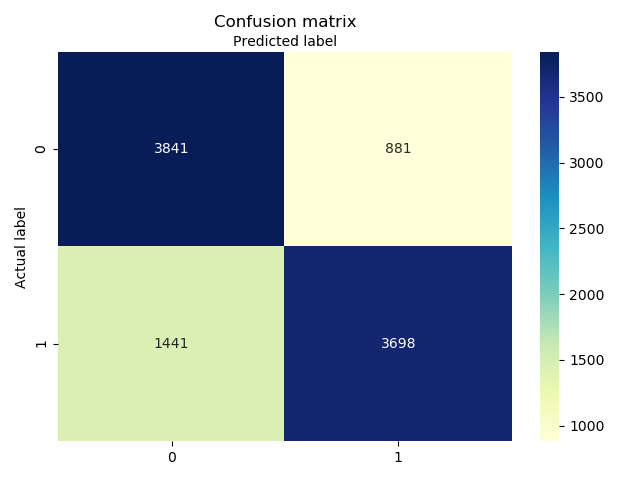
\includegraphics[scale=0.7]{Logistic_Regression}
\end{center}
This has an accuracy of 0.76 and a precision of 0.81.
\subsection{Decision Tree}
Decision tree classifiers work by looking at all the decisions that can be made, an example of a decision in this context is all the qualifications. A tree is then generated which can then be followed when forming predictions.\\
\\
With the Decision tree classifier the following confusion matrix was generated
\begin{center}
	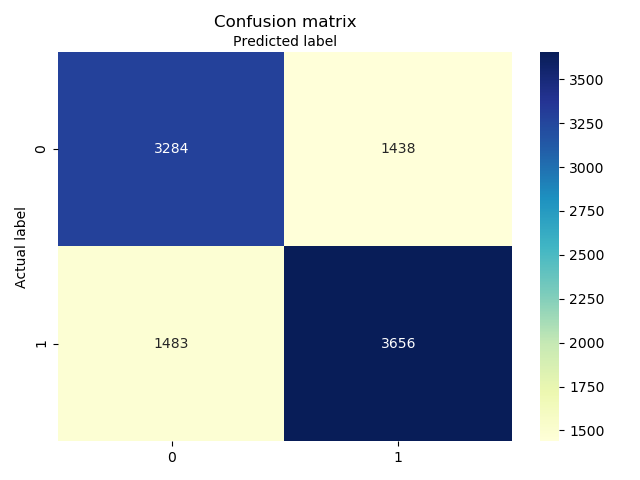
\includegraphics[scale=0.7]{Decision_Tree}
\end{center}
This has an accuracy of 0.70 and a precision of 0.72
\section{Conclusion}
In conclusion on this data set logistic regression has delivered better results, both in terms of accuracy and precision. Number of clicks in the VLE was the best predictor of performance I found, although other features also provide some predictive capacity.






\end{document}